% CALC14b
% Exploited Nicolini BH2-Pruefung Beamer Classes Sven
\documentclass[xcolor=dvipsnames]{beamer}


\usepackage[utf8]{inputenc}
\usepackage{hyperref}
\usepackage{amsmath}
\usepackage{cite}
\usepackage{units} % nicefrac
\usepackage{datetime} % fuer Uhrzeit im \date
\usepackage{wrapfig} % bilder rechts
\usepackage{caption} % fuer subcaption
\usepackage{subcaption} % subfigures
\usepackage{booktabs} % tables
\usepackage{mathtools} % right cases
\usepackage{color}

% Schriften
% Palatino for rm and math | Helvetica for ss | Courier for tt


%%\usepackage{mathpazo} % math & rm
%%\linespread{1.05}        % Palatino needs more leading (space between lines)
%%\usepackage[scaled]{helvet} % ss
%%\usepackage{courier} % tt
%%\normalfont
%%\usepackage[T1]{fontenc}

% Hyperref aufsetzen
\hypersetup{
    pdftitle={Sven Köppel Talk Journal Club Quantum Gravity FIAS Frankfurt Jun 2014},
    pdfauthor={Sven Köppel},
    pdfsubject={fias},
    pdfkeywords={physik} {black holes} {uni} {frankfurt},
    colorlinks=false,        % test: stat gerahmten Links
    linkcolor=red,          % color of internal links
    citecolor=darkgreen,    % color of links to bibliography
    filecolor=darkred,      % color of file links
    urlcolor=cyan           % color of external links
}

% Allgemeine Meta-Daten, genutzt fuer titlepage
\title{Some notes on calculating GUP/NCBHs in LXDs}
%\subtitle{and the issue of Particles in Curved Space}
\institute{Institut für theoretische Physik \\ Frankfurt Institute for Advanced Sciences \\ Goethe-Universität Frankfurt}
\author{\href{https://fias.uni-frankfurt.de/~koeppel}{Sven Köppel}\\
\small \texttt{koeppel@fias.uni-frankfurt.de}}
\date{Journal Club in High Energy Physics \\ Wed. 18. Jun 2014  \\ \gray \small Calc-15b} %\today, \currenttime}

% Beamerclasses theme waehlen

\usetheme[compress]{Singapore}
\usecolortheme{orchid}
%\usetheme[compress]{fiasbeamer/beamerthemefias}

% KLAPPT NICHT: 
%\usepackage{tikz}
%\usetikzlibrary{calc}
%\usetheme{fias}

\setbeamertemplate{footline}[frame number]
\beamertemplatenavigationsymbolsempty

% Hack um Subtitles als Frametitles zu nutzen,
% Bulletpoint fuer jede slide

\addtobeamertemplate{frametitle}{\let\insertframetitle\insertsubsectionhead}{}
\makeatletter
  \CheckCommand*\beamer@checkframetitle{\@ifnextchar\bgroup\beamer@inlineframetitle{}}
  \renewcommand*\beamer@checkframetitle{\global\let\beamer@frametitle\relax\@ifnextchar\bgroup\beamer@inlineframetitle{}}
\makeatother

% abgefahrenes highlighting von formeln
\usepackage{xcolor}
% klappt net, was einfacheres:
\newcommand{\highlight}[1]{%
  \colorbox{green!30}{$\displaystyle#1$}}


% MATH
\renewcommand{\d}{\mathrm{d}}
\newcommand{\dd}[2]{\frac{\mathrm{d} #1}{\mathrm{d} #2}}
\newcommand{\pp}[2]{\frac{\partial #1}{\partial #2}}
\renewcommand{\L}{L_P}
\newcommand{\pr}{p_r}
\newcommand{\psenk}{p_\perp}
\newcommand{\ebenso}{\biggl( ~ \therefore ~ \biggr) }
\newcommand{\metrik}[1]{\d s^2 = \left( #1 \right) \d t^2 \left( #1 \right)^{-1} \d r^2 + r^2 \d \Omega_{D-2}^2 }
\newcommand{\winkel}{r^2 \d \Omega^2}
\newcommand{\dann}{$\rightarrow~$}
\newcommand{\CA}{ {\cal A}}
\newcommand{\C}[1]{ {\cal #1}}
\newcommand{\mn}{_{\mu\nu}}

% colored symbols:
% http://tex.stackexchange.com/questions/85033/colored-symbols
\newcommand*{\mathcolor}{}
\def\mathcolor#1#{\mathcoloraux{#1}}
\newcommand*{\mathcoloraux}[3]{%
  \protect\leavevmode
  \begingroup
    \color#1{#2}#3%
  \endgroup
}
% In Text: $a\textcolor{red}{\ast}b$
% In Math: $a\mathcolor{red}{\ast}b$
\newcommand{\redmin}{\mathcolor{red}{-}}
\newcommand{\redplus}{\mathcolor{red}{+}}
\newcommand{\pn}{\mathcolor{red}{+ n}}
\newcommand{\n}{ {\mathcolor{red}{n}} }

% Gray out parts in equations
\newcommand{\gray}{ \color{gray} }
\newcommand{\black}{ \color{black} }

% Gelbe box ohne Extraplatz
% http://tex.stackexchange.com/questions/23681/colorboxcolortext-without-increasing-the-height-and-width-of-the-cell-in-a
\newcommand{\gelb}[1]{ {\setlength{\fboxsep}{0pt}\colorbox{yellow}{$#1$}} }
\newcommand{\green}[1]{ {\setlength{\fboxsep}{0pt}\colorbox{green}{$#1$}} }
\newcommand{\plus}{\gelb{+}}
\newcommand{\minus}{\green{-}}
\newcommand{\even}{\mathcolor{Violet}{even}}
\newcommand{\odd}{\mathcolor{Violet}{odd}}

% placeholder chars
\newcommand{\bul}[1]{ {\mathord{\color{#1!55}\bullet}} }

% Colors of plot
\definecolor{MathYellow}{RGB}{170, 170, 0}
\definecolor{MathMagenta}{RGB}{170, 0, 170}
\definecolor{MathBlue}{RGB}{230,230,255}

\newcommand*\itemL{\item[{
\includegraphics[height=2.5ex]{plots/bullet-L.pdf}}]}
\newcommand*\itemR{\item[{
\includegraphics[height=2.5ex]{plots/bullet-R.pdf}}]}
\newcommand*\itemDark{\item[{
\includegraphics[height=2.5ex]{plots/bullet-Dark.pdf}}]}
\newcommand*\itemLight{\item[{
\includegraphics[height=2.5ex]{plots/bullet-1.pdf}}]}


\begin{document}

\frame{\titlepage} 

%\frame{\frametitle{Inhaltsverzeichnis}\tableofcontents} 

\section{Technicalities: Cauchy theorem}
\subsection{The Fourier integral, 3 dimensions}
\begin{frame}
% Ablaufsteuerung:
%   http://mo.mathematik.uni-stuttgart.de/kurse/kurs44/seite38.html
% Wirkliches Einfaerben:
%   ftp://ftp.tex.ac.uk/tex-archive/info/math/voss/mathCol/mathCol.pdf
\begin{flalign*}
\int \d^3 p~f(p)~e^{i \vec x \vec p}
&= \int_0^{2\pi} \d \varphi
&& \int_0^\pi \d \theta \sin \theta
&& \int_0^\infty \d p~p^2~f(p)~e^{i\vec x \cdot \vec p} \\
%
&\gray = 2\pi 
&& \int_\gelb{-1}^\gelb{+1} \d \mathcolor{OliveGreen}{\cos \theta}
&&\gray \int_0^\infty \d p~p^2~f(p)~e^{\black i x p \mathcolor{OliveGreen}{\cos \theta}} \\
%
&= \gray 2\pi 
&& \int_0^\infty
\frac{1}{i x p}
&& \gray \d p~p^2~f(p)~
\black\left( e^{\gelb{+}i x p} - e^{\gelb{-}i x p}\right) \\
\end{flalign*}
\end{frame}

\subsection{The 3d Fourier integral $\to$ effective 1d}
\begin{frame}
\begin{align*}
% Problem: Zu wenig platz links! arghl
%\C F_3 \left\{ f(p) \right\}
\dots
&= \frac{2\pi}{ix} \int_0^\infty \d p~p
~f(p)~\Big( e^{\plus i x p} 
&& \minus ~ e^{\minus i x p}\Big)
\\
&= \gray \frac{2\pi}{ix}
\gray \Bigg(
{\gray \int_0^\infty \d p~p~f(p)}~e^{\plus ixp}
&& \minus 
{\gray \int_0^\infty \d p~p~f(p)}~e^{\minus ixp}
\gray \Bigg)
\\
&= \gray \frac{2\pi}{ix}
\gray \Bigg(
{\gray \int_0^\infty \d p~p~f(-p)}~e^{\plus ixp}
&&\plus
\overbrace{
\int_{\minus \infty}^0 \d p'~p'~f(\minus p')~e^{\plus ixp'}
}^{
\int_a^b = \minus \int_b^a
\quad\text{and}\quad
p' = \minus p}
\gray \Bigg)
\\
&=\mathrlap{ % macht Colspan!
\gray \frac{2\pi}{ix}
\black
\int_{\minus\infty}^{\plus\infty}
\d p~p~
\underbrace{
\Big[f(p) \Theta(p) + f(-p) \Theta(-p) \Big]
}_{=f(|p|)}
e^{\plus i x p}
} % end of mathrlap
\end{align*}

And $\gray \int \d p~\black p~f(|p|) \gray e^{ixp} \black \in \mathbb{C} \setminus \mathbb{R}
\quad \Rightarrow \quad i \int \dots \in \mathbb{R}$  \textcolor{OliveGreen}{\checkmark}
\end{frame}

\subsection{Does the same hold also in $3+n$ dimensions? $n\in \mathbb{N}_0$}
\begin{frame}
\begin{align*}
\int \d^{3\pn} f(p) e^{i \vec x \vec p}
&\propto \int_0^\infty \frac{1}{i x p} \d p~p^{2\pn}
~f(p)~\left( e^{\plus i x p} - e^{\minus i x p} \right)
\\
&\propto \int_{-\infty}^\infty \d p~
\underbrace{
p^{1\pn}
\Big[
f(p) \Theta(p)
+ \mathcolor{red}{(-1)^n} f(-p) \Theta(-p)
\Big]
}_{:= v(p)}
e^{\plus i x p}
\end{align*}
Spherical coordinates: \textcolor{OliveGreen}{\checkmark} \\
Effective 1d notation: \textcolor{OliveGreen}{\checkmark} \\
Issue with Holomorphy? \textcolor{YellowOrange}{Perhaps} \\
$\mathbb{R}$eal result? \textcolor{OliveGreen}{\checkmark}
\begin{itemize}
\item Even $n=0,2,4$: $v(p)=p^{\odd}f(|p|) \Rightarrow \int \in \mathbb{C}\setminus\mathbb{R} \Rightarrow
i \int \in \mathbb{R}$
\item Odd $n=1,3,5$: $v(p)=p^{\even} \Big[ \odd \Big] \Rightarrow \int \in \mathbb{C}\setminus\mathbb{R}
\Rightarrow i \int \in \mathbb{R} $
\end{itemize}
\end{frame}

\subsection{The $\Theta$ composition issue}
\begin{frame}
\begin{picture}(320,250)
\put(-25,15){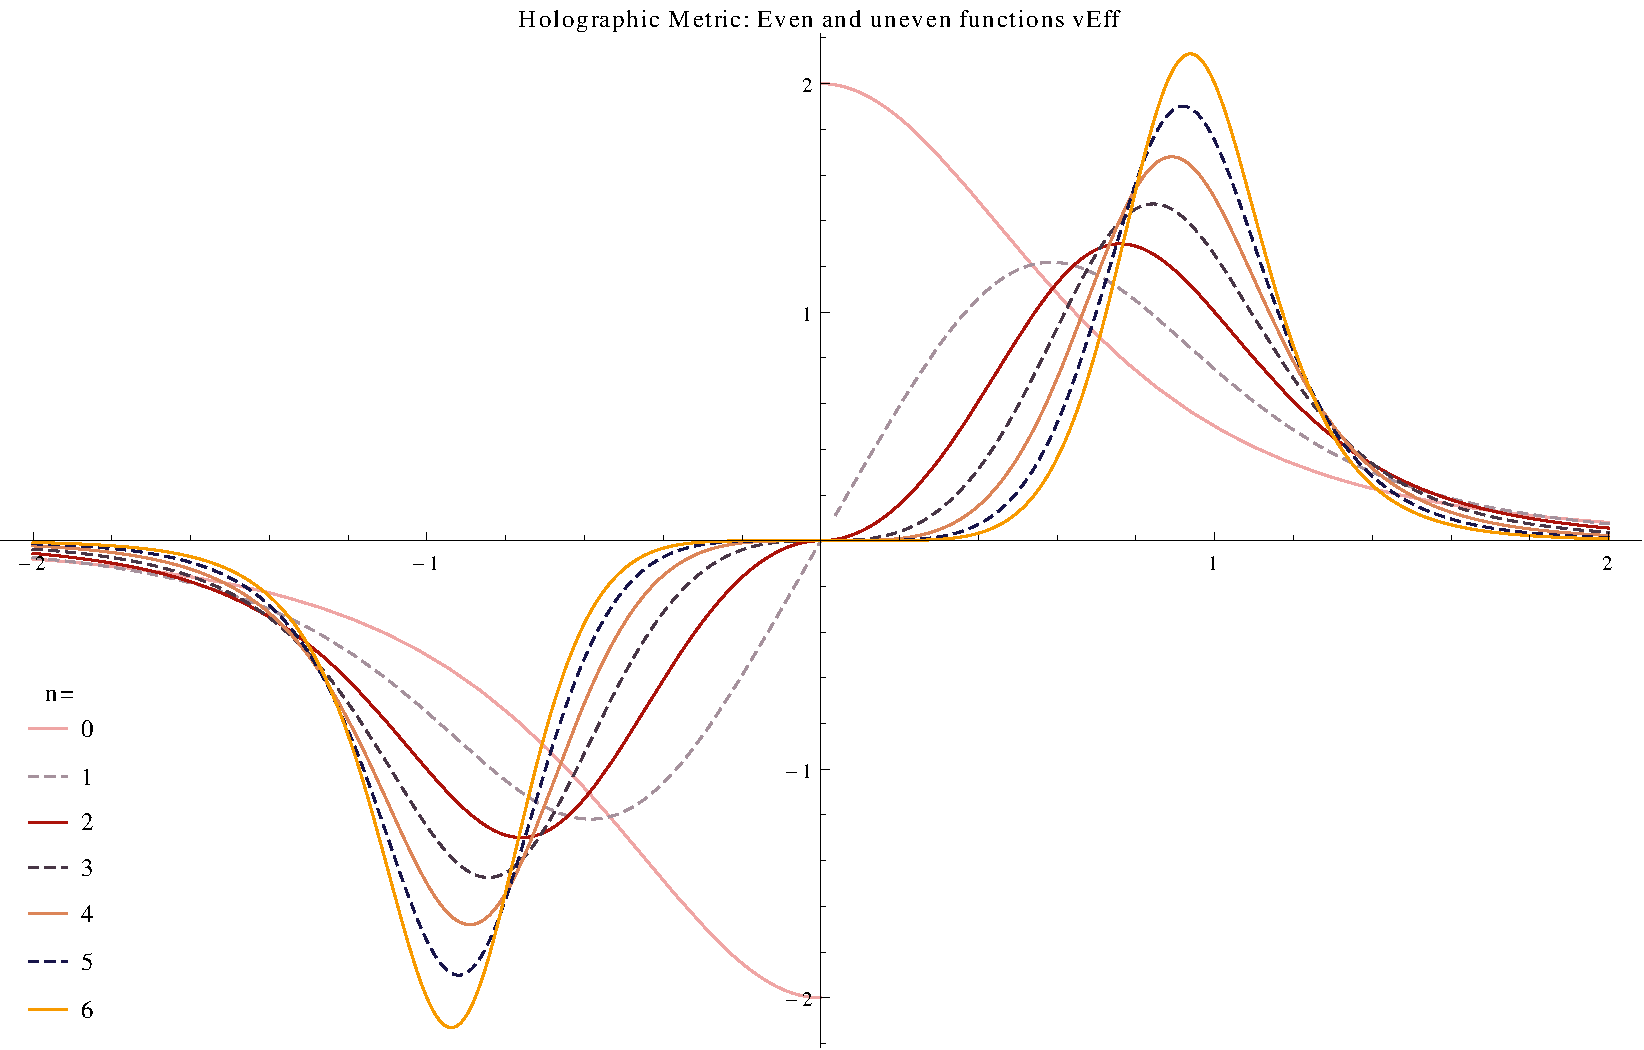
\includegraphics[width=\paperwidth]{plots/Holo-Calc13-vEff} }
\put(0,200){\begin{minipage}[t]{0.5\linewidth}
Example: Holographic metric
\begin{align*}
h(r) &= \frac{r^{2\pn}}{L^{2\pn} + r^{2\pn}} \\
\end{align*}
\end{minipage}}
\put(150,120){\begin{minipage}[t]{0.5\linewidth}
\begin{align*}
f(z) &= h'(z=r/L) \\
&= \frac{(2\pn) z^\n}{\left(z^{2\pn}+1\right)^2}
\end{align*}
\end{minipage}}
\end{picture}
\end{frame}

\subsection{Ignoring facts: Applying Cauchy theorem}
\begin{frame}
All $f(p)$ choices look roughly like
\begin{equation*}
f(p) \approx \frac{1}{
\left( 1 + L^\bul{red} p^\bul{red} \right)^\bul{blue}}
= \frac{1}{\left( 1 + q^\bul{red} \right)^\bul{blue}}
\end{equation*}
All $(\bul{red}-1)$ Poles are on the unit circle ($1=e^{i\varphi}$):
\begin{equation*}
q = (-1)^{\frac{1}{\bul{red}}} = \exp \left\{
\frac{i\pi + 2\pi i k}{\bul{red}}
\right\} \forall k \in \mathbb{N}
\end{equation*}
$\Rightarrow$ It's simple to sketch the setting!
\end{frame}

\subsection{From the complex plane...}
\begin{frame}
\begin{picture}(320,250)
\put(-30,15){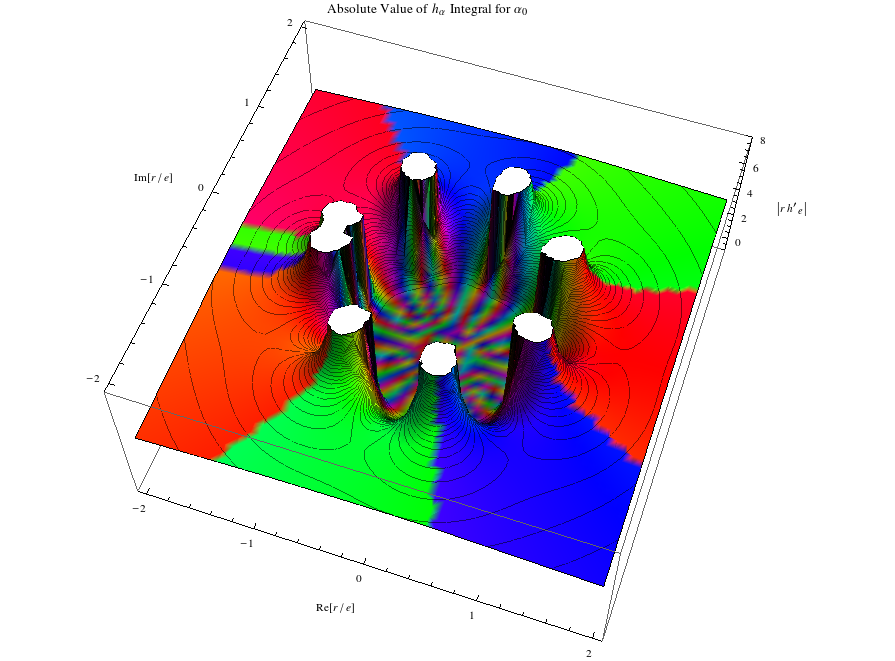
\includegraphics[width=0.85\paperwidth]{plots/Calc12-Symmetrie_fuer_Bardeen-Plot_hAlpha_n7.png}}
\put(180,230){\begin{minipage}[t]{0.5\linewidth}
Example: Self-encoding metric \\
{\tiny \textcolor{gray}{(The labeling lies: $r/e$ should be $r/L$)}}
\end{minipage}}
\put(190,110){\begin{minipage}[t]{0.5\linewidth}
\begin{align*}
h_\alpha(r) &= \frac{r^{3\pn}}{\left( r^\alpha + L^\alpha / 2 \right)^{3 \pn / \alpha}}
\end{align*}
\end{minipage}
}
\end{picture}
\end{frame}

\subsection{...to the pole diagram}
\begin{frame}
\begin{picture}(320,250)
\put(-10,35){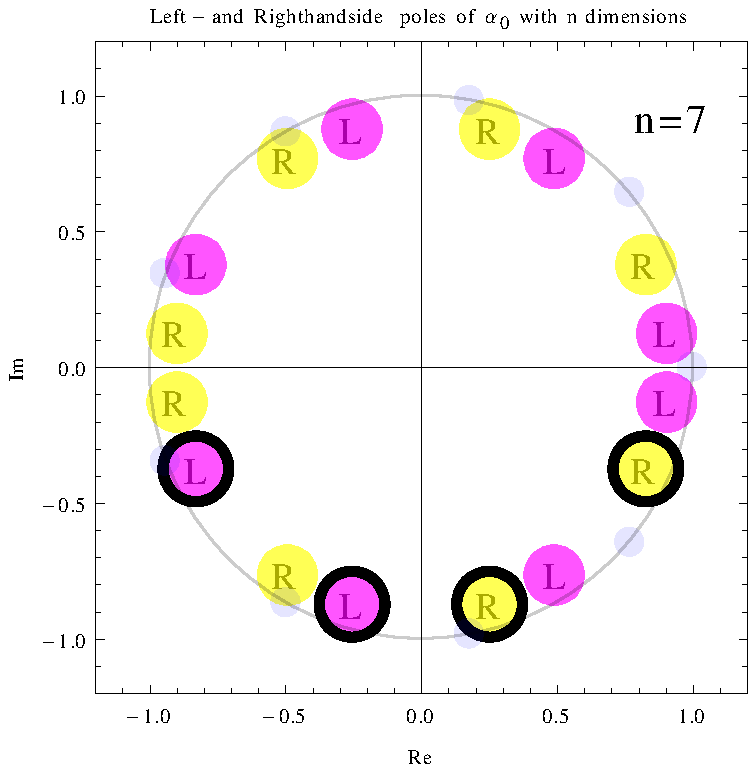
\includegraphics[width=0.48\paperwidth]{plots/Calc12-Symmetrie_fuer_Bardeen-Plot_hDiag-n7.pdf}}
\put(190,230){\begin{minipage}[t]{0.4\linewidth}
\begin{block}{Complex Points}
\begin{itemize}
\itemL Poles of $f(-p)$
\itemR Poles of $f(p)$
\itemDark Chosen poles
\itemLight Roots of unity
\end{itemize}
\end{block}

Only work left:
\begin{align*}
\int \d z = \sum \operatorname{Res}_{z\to z_0}
\end{align*}
\end{minipage}
}
\end{picture}
\end{frame}

\subsection{Results: Work must be checked}
\begin{frame}
\begin{itemize}
\item
Correct for no extra dimensions ($n=0$).
\item
Complex values do not vanish $\to$ Complex masses.
\end{itemize}
\end{frame}

\end{document}
